\section{Triangle systems on six labels}\label{sec:six-labels}

We now extract the finite combinatorial consequences of the equality case.
We call a face with three vertices a \emph{triangle}, and a face with four
vertices a \emph{tetrahedron}. These names refer to faces of the support
complex, not to geometric simplices in projective space.
Our eventual application is to the six labels complementary to a
tetrahedral facet of the ten-label support complex.

\begin{definition}\label{def:six-system}
A \emph{six-label triangle system} on a set $C$ of cardinality six is a
collection $\mathcal T\subseteq\binom{C}{3}$ such that
\begin{enumerate}
\item exactly one of $T$ and $C\setminus T$ belongs to $\mathcal T$ for
      each $T\in\binom{C}{3}$;
\item every pair of elements of $C$ belongs to exactly two members of
      $\mathcal T$.
\end{enumerate}
\end{definition}

\begin{lemma}\label{lem:six-from-map}
The triangles of the support complex of an admissible map
$f:\mathbb{RP}^2\to\Delta^5$ form a six-label triangle system.
\end{lemma}

\begin{proof}
By Theorem~\ref{thm:equality-complex}, the complex is pure of
dimension two, has all fifteen edges, and each edge belongs to a positive
even number of triangles. Two complementary triples cannot both be
triangles: choose witness lines $x,y\subset\mathbb R^3$ whose supports
contain the respective triples. A line perpendicular to both exists and,
by admissibility, could use none of the six labels.

There are ten complementary pairs of triples, so there are at most ten
triangles. Counting incidences between triangles and edges gives at least
$2\cdot15/3=10$ triangles. Equality holds throughout: there is one triangle
in each complementary pair, and every edge occurs twice.
\end{proof}

For a triangle system $\mathcal T$ on $C$ and $a\in C$, its \emph{link
graph at $a$} has vertex set $C\setminus\{a\}$ and an edge $\{u,v\}$
precisely when $\{a,u,v\}\in\mathcal T$.

\begin{lemma}\label{lem:six-properties}
Let $\mathcal T$ be a six-label triangle system on $C$.
\begin{enumerate}
\item Every vertex link is a cycle of length five.
\item Every four-element subset of $C$ contains a triangle, but does not
      contain all four of its triples as triangles.
\item If $a,b\in C$ are distinct and $R\subset C\setminus\{a,b\}$ has
      cardinality three, the link graphs at $a$ and $b$, restricted to $R$,
      are different. In particular, no transposition of two labels
      preserves $\mathcal T$.
\item The triangles contained in any five-element subset of $C$
      determine $\mathcal T$ uniquely.
\end{enumerate}
\end{lemma}

\begin{proof}
Every vertex of the link at $a$ has degree two, since the corresponding
pair with $a$ lies in exactly two triangles. A simple graph in which every
vertex has degree two is a disjoint union of cycles of length at least
three. On five vertices it must therefore be a single five-cycle.

Let $A\subset C$ have four elements and choose $a\in A$. A five-cycle
has no independent set of size three: if three vertices were independent,
the three gaps following them around the cycle would each contain another
vertex, requiring at least six vertices. Thus the other three elements of
$A$ contain an edge of the link at $a$, giving a triangle in $A$. If all
four triples in $A$ were triangles, the link at $a$ would contain the
three-cycle on $A\setminus\{a\}$, which a five-cycle cannot contain.

For the third assertion, write
$C=\{a,b,c,d,e,f\}$, where the two triangles containing $\{a,b\}$ are
$\{a,b,c\}$ and $\{a,b,d\}$. Deleting $b$ from the five-cycle at $a$
leaves a path on $\{c,d,e,f\}$ with endpoints $c,d$. Its middle edge is
$\{e,f\}$, so its other two edges are one of the matchings
\[
 M_1=\bigl\{\{c,e\},\{d,f\}\bigr\},\qquad
 M_2=\bigl\{\{c,f\},\{d,e\}\bigr\}.
\]
Deleting $a$ from the link at $b$ gives a path with the same endpoints
and middle edge. The two paths must use opposite matchings, as in
Figure~\ref{fig:six-label-paths}. For example,
if the first uses $M_1$, the triangles $\{a,c,e\}$ and $\{a,d,f\}$
exclude their complementary triples $\{b,d,f\}$ and $\{b,c,e\}$,
forcing the second path to use $M_2$.

The symmetric difference of the two paths is the four-cycle with edges
$M_1\cup M_2$. Every three of its four vertices retain an edge, so the
restrictions of the paths to any such triple differ. A transposition
$(a\ b)$ preserving the triangle system would make the two restricted
link graphs identical, which is impossible.

Finally, if $z$ is the omitted vertex of a five-element subset, every
triple containing $z$ has its complementary triple in that subset.
The complementary-triple rule therefore recovers its membership in
$\mathcal T$.
\end{proof}


\begin{figure}[tbp]
\centering
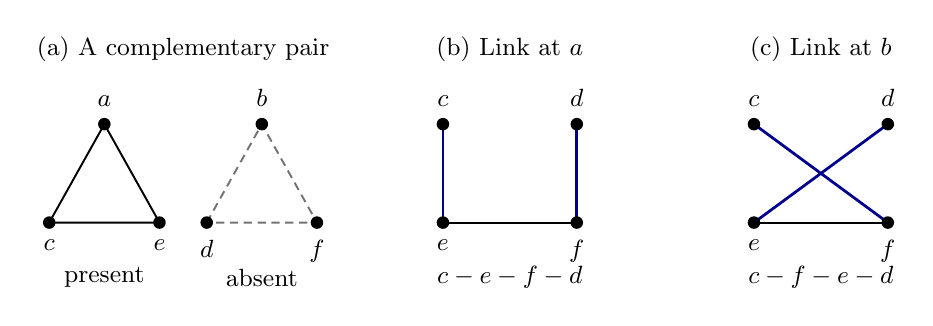
\begin{tikzpicture}[
  x=1cm,y=1cm,font=\small,
  vertex/.style={circle,fill=black,inner sep=1.6pt},
  every path/.style={line width=.7pt},
  matching/.style={draw=blue!55!black,line width=1pt}
]
\node at (1.7,2.2) {(a) A complementary pair};
\node at (5.85,2.2) {(b) Link at $a$};
\node at (9.8,2.2) {(c) Link at $b$};
\draw (0,0)--(.7,1.25)--(1.4,0)--cycle;
\node[vertex,label=above:$a$] at (.7,1.25) {};
\node[vertex,label=below:$c$] at (0,0) {};
\node[vertex,label=below:$e$] at (1.4,0) {};
\draw[densely dashed,draw=black!55] (2,0)--(2.7,1.25)--(3.4,0)--cycle;
\node[vertex,label=above:$b$] at (2.7,1.25) {};
\node[vertex,label=below:$d$] at (2,0) {};
\node[vertex,label=below:$f$] at (3.4,0) {};
\node at (.7,-.7) {present};
\node at (2.7,-.7) {absent};
\draw (5,0)--(6.7,0);
\draw[matching] (5,1.25)--(5,0) (6.7,0)--(6.7,1.25);
\node[vertex,label=above:$c$] at (5,1.25) {};
\node[vertex,label=above:$d$] at (6.7,1.25) {};
\node[vertex,label=below:$e$] at (5,0) {};
\node[vertex,label=below:$f$] at (6.7,0) {};
\node at (5.85,-.7) {$c-e-f-d$};
\draw (8.95,0)--(10.65,0);
\draw[matching] (8.95,1.25)--(10.65,0) (8.95,0)--(10.65,1.25);
\node[vertex,label=above:$c$] at (8.95,1.25) {};
\node[vertex,label=above:$d$] at (10.65,1.25) {};
\node[vertex,label=below:$e$] at (8.95,0) {};
\node[vertex,label=below:$f$] at (10.65,0) {};
\node at (9.8,-.7) {$c-f-e-d$};
\end{tikzpicture}
\caption{The complementary-triple rule forces opposite matchings.
Suppose the two triangles through $\{a,b\}$ are $\{a,b,c\}$ and
$\{a,b,d\}$. The links at $a$ and $b$, restricted to
$\{c,d,e,f\}$, share the edge $\{e,f\}$ and use opposite matchings
between $\{c,d\}$ and $\{e,f\}$ (shown in blue).
One of the two possible choices is drawn. The crossing in (c) is not a
vertex. Panel (a) shows one complementary pair for this choice.}
\label{fig:six-label-paths}
\end{figure}

